%%%%%%%%%%%%%%%%%%%%%%%%%%%%%%%%%%%%%%%%%%%%%%%%%%%%%%%%%%%%%%%%%%%%%%%%
\chapter{Fundamentals}
\label{sec:fundamentals}
%%%%%%%%%%%%%%%%%%%%%%%%%%%%%%%%%%%%%%%%%%%%%%%%%%%%%%%%%%%%%%%%%%%%%%%%

In diesem Kapitel werden die theoretischen Grundlagen und alle in der Arbeit verwendeten und für das Verständnis relevante Begriffe erläutert. Kapitelnamen spezifizieren, anpassen an die Fragestellung der Arbeit.

\makeatletter\ifthesis@masterthesis
Nach dem Lesen dieses Kapitels sollten folgende Punkte klar dargestellt sein:
\begin{itemize}
	\item Beschreibung der relevanten theoretischen Grundlagen für die Behandlung der Fragestellung
	\item Detaillierte Beschreibung ggf. vorhandener relevanter Spezifika des Anwendungsbereichs, in dem das Problem gelöst wird
	\item Detaillierte Beschreibung relevanter Spezifika eingesetzter Technologien
	\item Analyse bestehender Ansätze/ Vorarbeiten: Literaturstudium, Analyse, Vergleich und Zusammenfassung bestehender Ansätze.
\end{itemize}
\fi\makeatother

Gerade im Bereich der Grundlagen wird viel Literatur zitiert -- Details zum Zitieren finden Sie im Kapitel \ref{sec:references}. Da keine Diplomarbeit so innovativ ist, dass sie nicht auf vorhandenes Wissen aufbaut und in ein entsprechendes Forschungsumfeld eingebettet ist, kommt an dieser Stelle der Literaturrecherche eine besondere Bedeutung zu. Als Daumenregel gilt, dass der aktuelle Stand der Wissenschaft in der Informatik üblicherweise durch Publikationen v.a. der letzten 2 – 4 Jahre repräsentiert wird.

\makeatletter\ifthesis@masterthesis
Beispielhaft einleitender Text an dieser Stelle:\\
Dieses Kapitel stellt Konzepte der Informationstheorie vor und liefert theoretische Grundlagen zu verdeckten Kanälen. Die verdeckte Kommunikation wird mit den verwandten Techniken der Steganographie und Kryptographie verglichen. Außerdem werden ein einfaches Fehlerkorrekturverfahren sowie die Grundlagen des HTTP-Protokolls beschrieben.
\fi\makeatother

%=======================================================================
\section{State of the Art}
%=======================================================================
\begin{samepage}

	\subsection{Teletype for Atom}
	Teletype for Atom\footnote{https://github.com/atom/teletype/issues/211} is a Project enabling editing files peer to peer. It is based on 	\cite{Oster:2006:DataconsistencyforP2Pcollaborativeediting} \cite{YuWeihai:2014} \cite{BriotUrsoShapiro:2016:HighResponsivenessGroupEditing}.
	With Teletype it is possible to edit files currently opened by the "host". The files are only persisted on the "host" not on all peers.\footnote{https://teletype.atom.io/}
	Therefore disconnecting from the network cuts off the editing workflow. It is not possible to access all the files in a project unless they are opened by the host. 
	\subsection{Visual Studio Live Share}
	Visual Studio Live Share\footnote{https://visualstudio.microsoft.com/de/services/live-share/}  is a plugin for Visual Studio Code and Visual Studio that enables sharing all files of a project loaded in the editor with someone else. In addition to that it enables sharing debugging sessions and ports opened by debugging sessions are forwarded to clients. As with Teletype for Atom files are only persisted on the "host"  
	\subsection{Multihack-Brackets}
	Multihack-Brackets\footnote{https://github.com/multihack/multihack-brackets} is a plugin for the Brackets editor. It enables sharing an entire folder structure. It requires a server. As of 13.3.2019 it is not possible to verify performance or functionality since joining a session just crashes the brackets editor. 
	\subsection{Codeshare}
	Codeshare\footnote{https://codeshare.io} is a web based collaborative editor. It is designed for interviews. The editor window offers syntax highlighting for a broad range of programming languages. One shared room always only contains a single file. 
	\subsection{Summary}
	Overall none of the current solutions have any considerations for dealing with an underlying version control system of a project.

In diesem Kapitel wird ein Überblick über bereits existierende Lösungen für die Problemstellung bzw. verwandte Problemstellungen gegeben. Dabei ist eine Klassifizierung der existierenden Lösungen empfehlenswert. Eine Analyse der Lösungen, nach Kriterien sortiert, sollte insbesondere auch die Defizite der existierenden Lösungen erläutern und damit insbesondere auch eine Begründung liefern, warum diese Lösungen für die Problemstellung der Arbeit nicht herangezogen werden können.

%-----------------------------------------------------------------------
\subsection{Unterkapitel}
%-----------------------------------------------------------------------

Bei der Verwendung von Gliederungsebenen gibt es Folgendes zu beachten:
\begin{itemize}
	\item Es sollten nicht mehr als 3 Gliederungstiefen nummeriert werden.
	\item Unterkapitel sind nur dann sinnvoll, wenn es auch mehrere Untergliederungen gibt. Ein Kapitel 2.1.1 sollte somit nur dann verwendet werden, wenn es auch 2.1.2 gibt.
	\item Oft ist es einfacher und besser verständlich, Aufzählungen als Text zu formulieren und somit weitere Gliederungsstufen zu vermeiden.
\end{itemize}

%-----------------------------------------------------------------------
\subsection{Abbildungen}
\label{sec:abbildungen}
%-----------------------------------------------------------------------

Beschreibungen zu Abbildungen und Tabellen stehen unter dem Bild. Jede Abbildung muss im Fließtext referenziert werden. In \LaTeX besitzen Abbildungen typischerweise Labels, welche zum referenzieren verwendet werden. Zudem plaziert \LaTeX die Abbildungen an geeigneten Stellen, was meistens auch wünschenswert ist. Falls das nicht gewünscht wird, kann es durch Optionen beeinflusst werden.

Abbildung \ref{fig:xxx} verdeutlicht  \dots\\
(siehe Abbildung \verb|\ref{<label>}|)

\begin{figure}
	\centering
	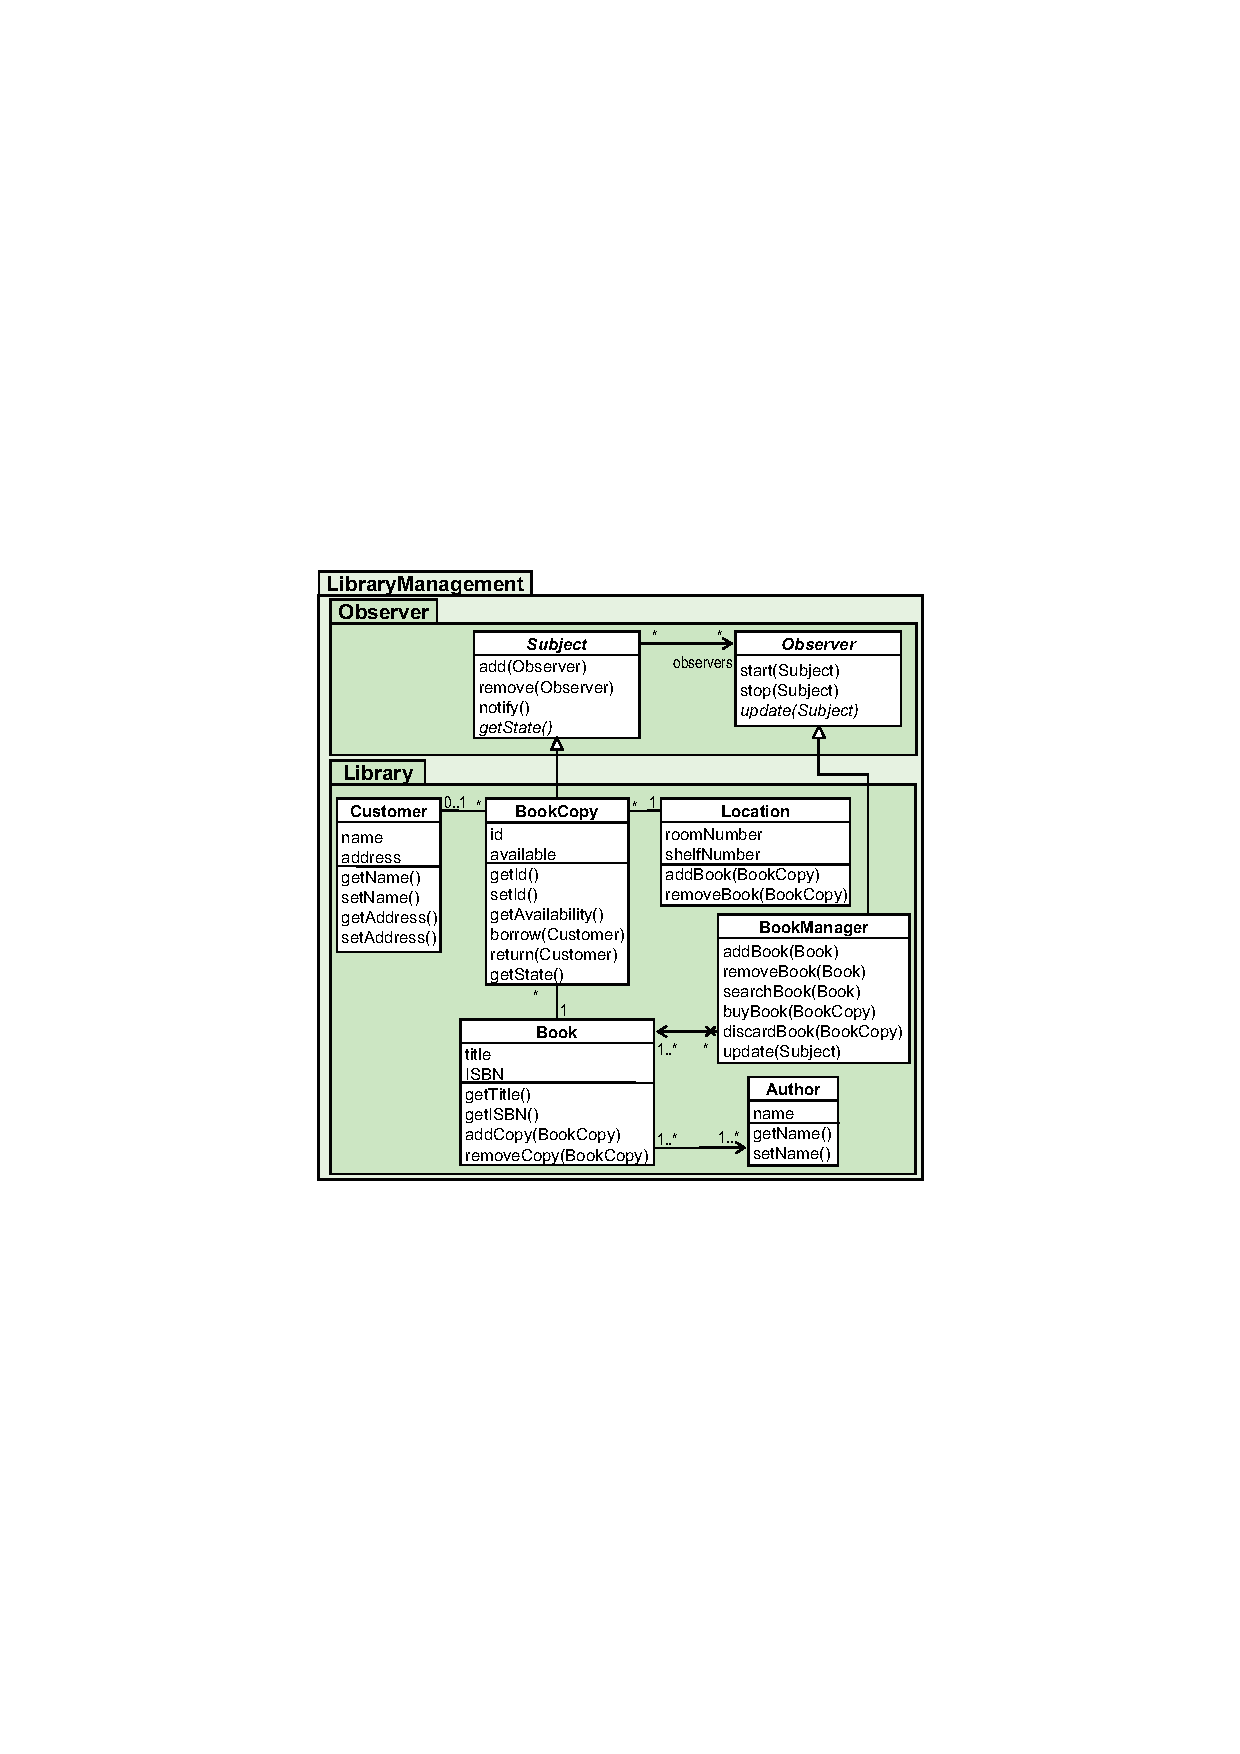
\includegraphics[width=0.4\linewidth]{figures/figure1}
	\caption{xxx (Quelle zitieren, wenn nicht selbst erstellt)}
	\label{fig:xxx}
\end{figure}

%-----------------------------------------------------------------------
\subsection{Tabellen}
%-----------------------------------------------------------------------

Jede Tabelle muss im Fließtext referenziertw werden. Für Tabellen gelten die selben Regeln, wie für Abbildungen (siehe dazu Abschnitt \ref{sec:abbildungen}).

Eine Beispiel einer Tabelle ist in Tabelle \ref{tab:xxx} zu finden:
\begin{table}
	\centering
	\begin{tabular}{| >{\bfseries}l | c | r | }
		\hline
			\rowcolor{orange} \bfseries Linksbündig & \bfseries Zentriert & \bfseries Rechtsbündig \\
		\hline
		\hline
			Zeile 1 & xxx & xxx \\\hline
			Zeile 2 & xxx & \dots \\\hline
			\multirow{2}{*}{Zeile3}
			& xxx & xxx \\\cline{2-3}
			& xxx & xxx \\\hline
		\hline
			\multicolumn{3}{| c |}{xxx} \\\hline
	\end{tabular}
	\caption{xxx (Quelle angeben)}
	\label{tab:xxx}
\end{table}

Bitte beachten Sie, dass Tabellen generell so einfach wie möglich gehalten werden sollen. Tabelle \ref{tab:xxx} dient unter anderem dazu Studierenden zu zeigen, wie Tabellen in \LaTeX\xspace erstellt werden können und wie Farben verwendet werden.